\documentclass[xetex,mathserif,serif]{beamer}
\usepackage{polyglossia}
\setdefaultlanguage[babelshorthands=true]{russian}
\usepackage{minted}
\usepackage{tabu}
\usepackage{pgfplots}
\usepackage{textpos}

\useoutertheme{infolines}

\usepackage{fontspec}
\setmainfont{FreeSans}
\newfontfamily{\russianfonttt}{FreeSans}

\usepackage{forest}
\usetikzlibrary{arrows}

\definecolor{links}{HTML}{2A1B81}
\hypersetup{colorlinks,linkcolor=,urlcolor=links}

\newcommand{\attribution}[1] {
\vspace{-5mm}\begin{flushright}\begin{scriptsize}\textcolor{gray}{\textcopyright\, #1}\end{scriptsize}\end{flushright}
}

\tabulinesep=0.7mm

\title{Абстрактные типы данных}
\author[Юрий Литвинов]{Юрий Литвинов \newline \textcolor{gray}{\small\texttt{yurii.litvinov@gmail.com}}}

\date{26.10.2018}

\begin{document}
	
	\frame{\titlepage}
	
	\begin{frame}
		\frametitle{АТД}
		\begin{itemize}
			\item АТД --- некоторая математическая модель и набор операций, определённый в рамках этой модели
			\begin{itemize}
				\item Обобщение понятия ``тип''
			\end{itemize}
			\item Состоит из типа данных и операций, выполняющих над ним преобразования
			\begin{itemize}
				\item Внутреннее устройство типа данных невидимо для остальной программы (принцип сокрытия деталей реализации)
				\item Работа с АТД --- только с помощью связанных с ним функций
				\item Тип данных и операции для работы с ним лежат в одном модуле, так, чтобы все изменения в АТД были локализованы и не затрагивали остальную программу (принцип инкапсуляции)
			\end{itemize}
			\item Дальнейшее обобщение АТД – классы
		\end{itemize}
	\end{frame}

	\begin{frame}
		\frametitle{Пример --- стек}
		\begin{itemize}
			\item stack.h / stack.cpp, при этом структура данных описана только в .cpp-файле, в .h-файле только её предварительное объявление
			\begin{itemize}
				\item Так компилятор может гарантировать сокрытие деталей реализации
				\begin{itemize}
					\item Всё, что не проверяется автоматически, можно считать не работающим!
				\end{itemize}
				\item Все функции принимают только указатель на структуру, для значения нужно знать размер
			\end{itemize}
			\item Функции:
			\begin{itemize}
				\item createStack()
				\item deleteStack()
				\item push()
				\item pop()
				\item isEmpty()
			\end{itemize}
			\item Внешнему миру вообще всё равно, как стек устроен внутри
			\begin{itemize}
				\item Может быть на массиве
			\end{itemize}
		\end{itemize}
	\end{frame}

	\begin{frame}[fragile]
		\frametitle{Ещё пример --- список}
		\begin{itemize}
			\item Требуется целых два типа --- сам список и позиция внутри списка
			\begin{itemize}
				\item Что-то вроде индекса элемента массива, но может быть устроена хитрее
				\item Позиция должна обеспечивать быструю работу с элементом, на который она указывает
				\item Внешнему миру всё равно, как устроен список и что такое позиция
				\begin{itemize}
					\item Может быть, список на массивах, а позиция --- число, или список на указателях, а позиция --- указатель на элемент списка (или даже на предыдущий элемент)
				\end{itemize}
			\end{itemize}
			\item Список может хранить разные типы элементов
			\begin{itemize}
				\item typedef --- ``шаблоны для бедных''
				\begin{itemize}
					\item 
					\begin{footnotesize}
						\begin{minted}{cpp}
typedef int Value;
struct ListElement { 
    Value value;
    ListElement *next;
}
						\end{minted}
					\end{footnotesize}
					\item typedef же может использоваться для описания типа позиции
				\end{itemize}
			\end{itemize}
		\end{itemize}
	\end{frame}

	\begin{frame}
		\frametitle{Инвариант}
		\begin{itemize}
			\item Некоторое логическое условие, верное всё время жизни АТД
			\begin{itemize}
				\item Не совсем, внутри функции АТД инвариант может нарушаться
				\begin{itemize}
					\item Не всегда, потому что бывают многопоточные программы
				\end{itemize}
			\end{itemize}
			\item АТД отвечает за поддержание своего инварианта
			\begin{itemize}
				\item Поскольку работа с АТД только через его функции, у внешнего мира нет способа его испортить
			\end{itemize}
			\item Пример --- размер списка
			\begin{itemize}
				\item Можно считать за $O(n)$ каждый раз
				\item Можно хранить как элемент структуры, тогда должен соблюдаться инвариант
			\end{itemize}
			\item Ещё пример --- head и tail у очереди
		\end{itemize}
	\end{frame}

	\begin{frame}
		\frametitle{Пример применения АТД --- сортировка слиянием}
		Если в списке больше одного элемента, делим его на два, вызываем mergesort, получаем два отсортированных списка, которые сливаем в один отсортированный
		\begin{columns}
			\begin{column}{0.6\textwidth}
				\begin{itemize}
					\item $O(n * log(n))$ в среднем и худшем случае
					\item Устойчива
					\item Внешняя (подходит для больших данных, не помещающихся в память)
					\item \url{http://www.ee.ryerson.ca/~courses/coe428/sorting/mergesort.html}
					\item Ей не надо знать внутреннего устройства списка
				\end{itemize}
			\end{column}
			\begin{column}{0.4\textwidth}
				\begin{center}
					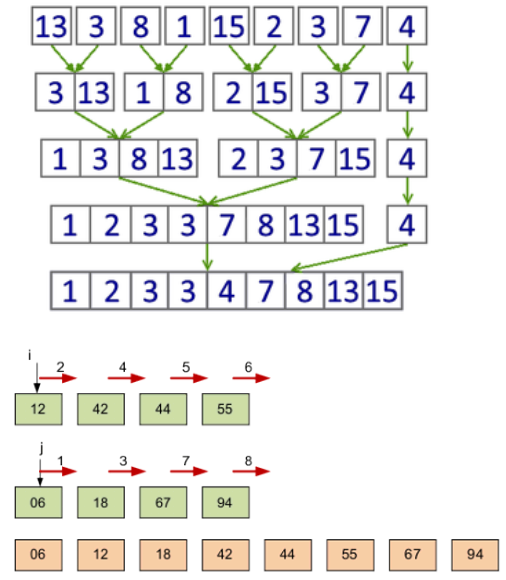
\includegraphics[width=0.95\textwidth]{mergesort.png}
				\end{center}
			\end{column}
		\end{columns}
	\end{frame}

	\section{Немного С++}

	\begin{frame}
		\frametitle{Немного С++}
		\begin{itemize}
			\item \mintinline{cpp}|vector<int> array(10);|
			\item \mintinline{cpp}|string str = "C++ roxx";|
			\item stack, queue, priority\_queue, ...
			\begin{itemize}
				\item Обратите внимание, STL (Standard Template Library, это оттуда все эти классы) не следует правилам стайлгайда
			\end{itemize}
			\item cin/cout
			\item Итераторы и умные указатели (только для тех, кто знает, что это)
		\end{itemize}
	\end{frame}

	\begin{frame}[fragile]
		\frametitle{Пример, чтение из файла}
		\begin{scriptsize}
			\begin{minted}{cpp}
#include <fstream>
#include <iostream>
#include <vector>
#include <string>

using namespace std;

int main()
{
    ifstream file("test.txt", ios::in);
    if (!file.is_open()) 
    {
    cout << "File not found!" << endl;
        return 1;
    }

    ...

    return 0;
}
			\end{minted}
		\end{scriptsize}
	\end{frame}

	\begin{frame}[fragile]
		\frametitle{Собственно, чтение}
		\begin{scriptsize}
			\begin{minted}{cpp}
int main()
{
    ...
    vector<string> data;

    while (!file.eof()) {
        string buffer;
        file >> buffer;
        data.push_back(buffer);
    }

    file.close();

    for (string const &line : data) 
    {
        cout << line << endl;
    }

    return 0;
}
			\end{minted}
		\end{scriptsize}
	\end{frame}

	\begin{frame}
		\frametitle{using namespace, what?}
		Карго-культ, также религия самолётопоклонников или культ Даров небесных --- термин, которым называют группу религиозных движений в Меланезии. В культах карго верят, что западные товары созданы духами предков и предназначены для меланезийского народа. Считается, что белые люди нечестным путём получили контроль над этими предметами. В культах карго проводятся ритуалы, похожие на действия белых людей, чтобы этих предметов стало больше.
		\attribution{Wikipedia}
	\end{frame}

	\begin{frame}[fragile]
		\frametitle{Пространства имён}
		\begin{minted}{cpp}
namespace namespace1 
{
    struct A 
    {
    }
}

namespace namespace2 
{
    struct A 
    {
    }
}
		\end{minted}
	\end{frame}

	\begin{frame}[fragile]
		\frametitle{using namespace}
		\begin{minted}{cpp}
using namespace namespace2;

int main()
{
    A a;
    namespace1::A a1;
}
		\end{minted}
	\end{frame}

\end{document}